%% estilo do documento e medidas
\documentclass[a4paper,portuguese,utf8,T1]{article}
\usepackage[top=3cm,bottom=2cm,left=2cm,right=2cm,marginparwidth=1.75cm]{geometry}
\usepackage{indentfirst}
\renewcommand{\baselinestretch}{1.2}
\setlength{\marginparwidth}{2cm}

%% linguagem e fontes
\usepackage[utf8]{inputenc}
\usepackage[T1]{fontenc}
\usepackage[portuguese]{babel}

%% referencias
\usepackage[
    backend = biber,
    style = alphabetic,
    sorting = ynt
]{biblatex}
\addbibresource{dados/referencias.bib}

%% pacotes para desenhos e ambientes diferenciadas
\usepackage{amsmath}						% símbolos e ambientes matemáticos
\usepackage{booktabs}						% tabelas melhoradas
\usepackage{datatool}						% recolhimento de dados
\usepackage[table,xcdraw]{xcolor}			% mais cores
\usepackage{graphicx}						% figuras melhoradas
\usepackage{subcaption}						% subfiguras
\usepackage[colorinlistoftodos]{todonotes}	% notas para a escrita
\usepackage[colorlinks,citecolor=blue]{hyperref}		% links
\usepackage{circuitikz}						% desenho de circuitos
\usepackage{csvsimple}						% dados em CSV
\usepackage{cleveref}						% referenciamento melhorado
\usepackage{multirow}						% tabelas de multíplas linhas ou colunas
\usepackage{float}							% fixar posição de figuras
\usepackage{csquotes}                       % aspas melhoradas

% unidades do SI
\usepackage[
	exponent-to-prefix = true,
	round-mode = figures,
	scientific-notation = engineering,
	zero-decimal-to-integer = false,
	separate-uncertainty = true,
	multi-part-units = single
]{siunitx}

% setup para usar o cleveref com o subcaption
% \captionsetup[subfigure]{subrefformat=simple,labelformat=simple}
%     \renewcommand\thesubfigure{(\alph{subfigure})}

%% dados do relatório
\title{
	\Huge Experimento 4 			\\
    \Large Física Experimental IV
}
\author{
	\small Grupo 3:					\\
	Felipe Mack (81335),			\\
    Gabriel Ferrauche (197314) e	\\
    Tiago de Paula (187679)
}
\date{\small\today}

%%%%%%%%%%%%%%%%%%%%%%%%%%%%%
%% Relatório, propriamente %%
%%%%%%%%%%%%%%%%%%%%%%%%%%%%%
\begin{document}

	%% Cabeçalho %%
	\maketitle

	%%%% Resumo %%%%
	\begin{abstract}
    	\textit{A decomposição da luz em ondas de diferentes frequências decorre da dependência do índice de refração de um material do comprimento de onda da onda incidente.

Neste experimento, foi medida a relação de dispersão de um prisma de vidro a partir dos ângulos de desvio mínimo decorrentes da decomposição da luz emitida por lâmpadas de Hélio (\ce{He}), Cádmio (\ce{Cd}), Mercúrio (\ce{Hg}) e Sódio (\ce{Na}). Partindo das medidas de ângulo de desvio mínimo, este experimento teve como objetivo anlisar a precisão deste deste aparato todo para medições desse tipo de natureza, utilizando como modelo a equação de Cauchy.

O resultado de tudo isso foi uma resolução espectral de \SI[detect-all = true]{32}{\nano\meter} na faixa de luz visível, capaz de diferenciar até 11 faixas distintas de comprimentos de onda nesse espectro. Isso já seria uma quantia razoável para esse equipamentos, porém eles têm potencial para muito mais se o modelo teórico for calibrado mais precisamente.
}
	\end{abstract}

	%%%%% Introdução %%%%%
	\section{Introdução} \label{introducao}
		Dentre todos os fenômenos ondulatórios, a difração possui uma posição de destaque. Sendo uma conclusão direta do princípio de Hyugens-Fresnel, em que uma frente de onda funciona como várias novas fontes, a difração da luz em conjunto com a refração foram as grandes afrontas à teoria corpuscular da luz, concedida por Isaac Newton.

Utilizando da difração, Thomas Young derrubou, no início do século XIX, a teoria da luz como partícula. Ao montar um experimento com duas fendas de difração, ele mostrou um exemplo de interferência luminosa, com interferências contrutivas e destrutivas, um fenômeno que não podia ser explicado pela teoria de Newton e provava a natureza ondulatória da luz.

Este experimento traz uma reconstrução de parte do experimento de Young, conhecido por “Experimento da Dupla Fenda”, bem como uma extensão dos resultados para a difração da luz em fendas simples, duplas e múltiplas.

Além da comprovação da natureza ondulatória da luz é possível determinar o comprimento de onda da luz incidente a partir dos padrões de interferência formados pela rede de difração.

Assim, este experimento tem como objetivos: observar os efeitos de difração em fendas simples e os efeitos de interferência em fendas simples e múltiplas; verificar as previsões do modelo de difração de Fraunhofer para fendas simples e sua validade para múltiplas fendas, comparando a medida da largura de uma fenda a partir de padrões de difração com a medida realizada com microscópio metrológico.



	%%%%% Materiais e Métodos %%%%%
	\section{Materiais e Métodos} \label{metodos}
    	Os materiais utilizados para o experimento foram: goniômetro, lâmpadas de diferentes elementos químicos, lupa e prisma de numeração 17.

para  o início da coleta de dados, o primeiro passo se resumiu a calibrar o goniômetro. Para tal, o prisma foi retirado do goniômetro, a luneta de leitura foi destravada e alinhada com com a entrada de luz da lâmpada de Sódio, travando a luneta. Na sequência, o foco da luneta foi ajustado de para que a cruz no interior da mesma pudesse ser visto de forma nítida, assim como a fenda de entrada de luz; o parafuso de ajuste fino foi empregado para garantir que a cruz se alinhasse com o lado fixo da fenda, \textbf{que possuia um ajuste de abertura}. Para finalizar o ajuste, o disco graduado do goniômetro foi liberado seu "zero" foi alinhado com o "zero" da luneta.



	%%%%% Resultados %%%%%
	\section{Resultados} \label{resultados}
	 	\begin{figure}[H]
    \centering

    \begin{subfigure}[t]{\textwidth}
        \centering
        \scalebox{2.5}{
            \begingroup
  \sbox{\tempbox}{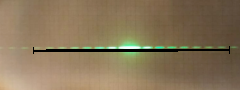
\includegraphics[width=\textwidth]{figuras/medidas/C4.pdf}}
  \begin{picture}(\wd\tempbox,\ht\tempbox)
    \put(0,0){\usebox{\tempbox}}
    \put(.502\wd\tempbox,.33\ht\tempbox){$8~\Delta y$}
  \end{picture}
\endgroup


        }
        \caption{C4}
        \label{fig:C4}
    \end{subfigure}
    \qquad
    \begin{subfigure}[t]{\textwidth}
        \centering
        \scalebox{5}{
            \begingroup
  \sbox{\tempbox}{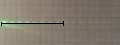
\includegraphics[width=\textwidth]{figuras/medidas/C5.pdf}}
  \begin{picture}(\wd\tempbox,\ht\tempbox)
    \put(0,0){\usebox{\tempbox}}
    \put(.22\wd\tempbox,.38\ht\tempbox){$4~\Delta y$}
  \end{picture}
\endgroup


        }
        \caption{C5}
        \label{fig:C5}
    \end{subfigure}
    \qquad
    \begin{subfigure}[t]{\textwidth}
        \centering
        \scalebox{5}{
            \begingroup
  \sbox{\tempbox}{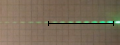
\includegraphics[width=\textwidth]{figuras/medidas/C6.pdf}}
  \begin{picture}(\wd\tempbox,\ht\tempbox)
    \put(0,0){\usebox{\tempbox}}
    \put(.47\wd\tempbox,.39\ht\tempbox){$20~\Delta y$}
  \end{picture}
\endgroup


        }
        \caption{C6}
        \label{fig:C6}
    \end{subfigure}

    \caption{C}
    \label{fig:C}
\end{figure}
\begin{figure}[H]
    \centering

    \begin{subfigure}[t]{\textwidth}
        \centering
        \scalebox{2.5}{
            \begingroup
  \sbox{\tempbox}{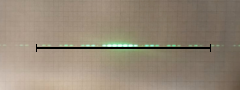
\includegraphics[width=\textwidth,page=1]{figuras/medidas/B4.pdf}}
  \begin{picture}(\wd\tempbox,\ht\tempbox)
    \put(0,0){\usebox{\tempbox}}
    \put(0,0){\includegraphics[width=\textwidth,page=2]{figuras/medidas/B4.pdf}}
    \put(.47\wd\tempbox,.37\ht\tempbox){$4~\Delta y$}
    \put(.48\wd\tempbox,.54\ht\tempbox){$5\Lambda$}
  \end{picture}
\endgroup


        }
        \caption{B4}
        \label{fig:B4}
    \end{subfigure}
    \qquad
    \begin{subfigure}[t]{\textwidth}
        \centering
        \scalebox{2.49}{
            \begingroup
  \sbox{\tempbox}{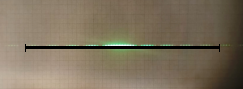
\includegraphics[width=\textwidth,page=1]{figuras/medidas/B5.pdf}}
  \begin{picture}(\wd\tempbox,\ht\tempbox)
    \put(0,0){\usebox{\tempbox}}
    \put(0,0){\includegraphics[width=\textwidth,page=2]{figuras/medidas/B5.pdf}}
    \put(.48\wd\tempbox,.37\ht\tempbox){$5~\Delta y$}
    \put(.46\wd\tempbox,.525\ht\tempbox){$11~\Lambda$}
  \end{picture}
\endgroup


        }
        \caption{B5}
        \label{fig:B5}
    \end{subfigure}
    \qquad
    \begin{subfigure}[t]{\textwidth}
        \centering
        \scalebox{2.5}{
            \begingroup
  \sbox{\tempbox}{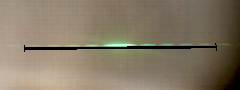
\includegraphics[width=\textwidth,page=1]{figuras/medidas/B6.pdf}}
  \begin{picture}(\wd\tempbox,\ht\tempbox)
    \put(0,0){\usebox{\tempbox}}
    \put(0,0){\includegraphics[width=\textwidth,page=2]{figuras/medidas/B6.pdf}}
    \put(.47\wd\tempbox,.38\ht\tempbox){$5~\Delta y$}
    \put(.595\wd\tempbox,.54\ht\tempbox){$6\Lambda$}
  \end{picture}
\endgroup


        }
        \caption{B6}
        \label{fig:B6}
    \end{subfigure}

    \caption{B}
    \label{fig:B}
\end{figure}


	%%%%% Discussão %%%%%
	\section{Discussão} \label{discussao}
    	A partir dos resultados observados na seção \ref{resultados}, a proximidade entre os valores obtidos a partir de cálculos, seguindo o modelo de Fraunhofer e aqueles obtidos com microscópio metrológico, é possível observar que o modelo citado demonstrou grande coerência. Os valores obtidos tanto para a largura das fendas quanto para a separação das mesmas foram condizentes para ambas as formas de medição, ou seja, demonstraram resultados similares. verificando a das previsões de Fraunhofer.

Para todos os conjuntos de fendas, de A a C, as grandezas mensuradas tiveram diferenças numéricas da ordem de micrômetros. Assim evidenciou-se que, pelo modelo de Fraunhofer é possível determinação da das grandezas das fendas de difração.

O experimento também demostrou, como pode ser visto na imagem x, que a largura dos máximos primários de interferência depende da quantidade de fendas, não apenas da largura e separação das mesmas. Novamente, mais um resultado que seria esperado, seguindo o modelo teórico.

Em relação às imagens observadas na figura \ref{fig:D}, as mesmas demonstraram que o padrão de difração observado no anteparo não so depende da largura, separação e quantidade de fendas, mas como também do formato e disposição das fendas. Assim, evidenciando que o padrões de difração e interferência observados podem ser muito diversos, dependendo fortemente das condições experimentais presentes, em especial, das características físicas das fendas.



    %%%%% Conclusão %%%%%
    \section{Conclusão} \label{conclusao}
    	Ao fim do experimento, concluiu-se que ambos filtros construídos pelo grupo forma extremamente eficazes para atingir os objetivos propostos. Também observou-se que os modelos teóricos empregados foram coerentes, dado que as frequências de corte e central calculadas corresponderam com exatidão com os dados coletados. Assim, mostrando coesão entre os modelos teóricos e o comportamento real do sistemas estudados.


	%%%%%% Referências %%%%%%
    \printbibliography

\end{document}